% ============================================================================
%  KRONOS — Academic Paper
%  Knowledge-Routed Neuro-Symbolic Multimodal Reasoning
%  for Faithful Chest X-ray VQA
% ============================================================================
\documentclass[runningheads]{llncs}

\usepackage[utf8]{inputenc}
\usepackage{graphicx}
\usepackage{booktabs}
\usepackage{amsmath,amssymb}
\usepackage{algorithm}
\usepackage{algorithmic}
\usepackage{tikz}
\usetikzlibrary{shapes.geometric,arrows.meta,positioning,fit,backgrounds,calc}
\usepackage{xcolor}
\usepackage{hyperref}
\usepackage{multirow}
\usepackage{subcaption}

\definecolor{symblue}{HTML}{1A5276}
\definecolor{visred}{HTML}{C0392B}
\definecolor{vergreen}{HTML}{1E8449}
\definecolor{caupurple}{HTML}{7D3C98}

\hypersetup{
  colorlinks=true,
  linkcolor=black,
  urlcolor=symblue,
  citecolor=symblue
}

\begin{document}

\title{KRONOS: Verifier-Guided Multimodal Tree Search\\for Faithful Chest X-ray Visual Question Answering}

\author{Gia Huy Nguyen \and Manh Cuong Vu}

\authorrunning{G.H. Nguyen, M.C. Vu}

\institute{University of Medicine and Pharmacy at Ho Chi Minh City, Vietnam}

\maketitle

% ============================================================================
\begin{abstract}
Medical Visual Question Answering (VQA) systems can produce correct answers
backed by wrong reasoning---a critical failure mode when clinicians cannot
audit \emph{why} a model reached its conclusion.
We present \textbf{KRONOS}, a neuro-symbolic VQA system for chest X-rays
that guarantees \emph{faithful, auditable evidence traces} by construction.
A frozen vision-language model (MedGemma 4B) acts as a search agent over a
tree of interleaved \emph{visual} actions (inspect, re-detect, compare) and
\emph{symbolic} actions (ontology traversal, closed-world negation, anatomy
mapping, causal graph exploration).
Unlike prior tree-search methods that rely on LLM self-evaluation as a value
function, KRONOS uses a \textbf{deterministic verifier} that scores nodes by
\emph{closure-progress}---the degree to which a provable reasoning path has
been established on a clinical knowledge graph.
The winning root-to-leaf path \emph{is} the evidence trace: symbolic steps
are sound on the DAG, visual steps cite auditable image regions, and
a \emph{deletion test} confirms that every step is causally necessary for
the answer.
For multi-hop reasoning, KRONOS adopts a Think-on-Graph paradigm: the VLM
explores causal edges on an RGO-derived knowledge graph while the verifier
decides when a shared-cause chain is established---yielding traces where
every edge is a real KG edge by construction.
Answers are tiered: \textbf{Tier~A} (faithful, verified), \textbf{Tier~B}
(advisory, flagged), or \textbf{Abstain} (insufficient evidence).
The entire pipeline is inference-only---no training---with frozen detector,
frozen VLM, and a CPU-only deterministic engine.

\keywords{Medical VQA \and Faithful reasoning \and Neuro-symbolic AI
\and Tree search \and Chest X-ray \and Knowledge graph}
\end{abstract}

% ============================================================================
\section{Introduction}
\label{sec:intro}
% ============================================================================

Radiologists read 60--100 chest X-rays (CXRs) per day, with a 3--5\%
diagnostic error rate that increases under workload
pressure~\cite{bruno2015error}.
AI-assisted Medical VQA---where a clinician poses natural-language questions
about a radiograph and receives automated answers---promises to reduce
missed findings and accelerate triage.
Yet current systems optimize \emph{answer accuracy} while ignoring
\emph{evidence faithfulness}: whether the answer was reached \emph{for the
right clinical reasons}.

Recent work has shown that chain-of-thought (CoT) traces produced by large
language models are often \emph{post-hoc rationalizations} rather than
faithful records of the reasoning process~\cite{turpin2023unfaithful,
arcuschin2025cot}.
In the medical domain, Moll et al.~\cite{moll2025evaluating}
demonstrated that when input images are perturbed, medical VLMs retain
identical explanations---evidence that the explanation does not reflect the
decision process.
This ``right answer, wrong reason'' failure mode is particularly dangerous
in clinical settings: if a clinician cannot verify the reasoning, they
cannot trust or correct the system.

We identify five gaps in existing approaches:
\begin{enumerate}
  \item \textbf{Unfaithful CoT.} LLM-generated explanations are post-hoc;
    no structural guarantee ties the trace to the answer.
  \item \textbf{Knowledge graphs at training, not inference.}
    MedReason~\cite{wang2025medreason} uses knowledge graphs to generate
    training data but discards them at inference---the fine-tuned LLM
    generates reasoning freely, with no graph-grounded guarantee.
  \item \textbf{LLM self-evaluation as value function.}
    LATS~\cite{zhou2024lats} and visual-MCTS methods use the LLM itself (or
    a learned reward model) to score search branches---an inherently
    unfaithful signal.
  \item \textbf{Linear reasoning cannot recover from errors.}
    ReAct~\cite{yao2023react} chains are one-shot: a wrong first step
    dooms the entire trace.
  \item \textbf{Multi-hop clinical reasoning lacks grounding.}
    Questions like ``Can one condition cause both findings A and B?'' require
    traversing causal pathways, but existing systems either hallucinate
    causal links or answer without traceable evidence chains.
\end{enumerate}

\textbf{KRONOS} addresses all five gaps with a single architectural
principle: \emph{verifier-guided multimodal tree search}.
A frozen VLM agent searches over a tree of interleaved visual and symbolic
actions, guided by a deterministic verifier whose reward measures
\emph{closure-progress} toward a provable path on a clinical ontology DAG.
The winning path is faithful by construction: symbolic steps are sound on
the graph, visual steps cite auditable image regions, and a deletion test
confirms causal necessity.
For multi-hop causal reasoning, the same engine adopts a Think-on-Graph
(ToG) paradigm~\cite{sun2024thinkongraph}: the VLM selects which causal
edges to explore on an RGO-derived knowledge graph~\cite{budovec2014rgo},
while the verifier---never the VLM---decides when the path is sufficient.

\noindent\textbf{Contributions.}
\begin{enumerate}
  \item A \textbf{verifier-as-value} tree search where the reward is
    deterministic closure-progress on a knowledge graph, replacing LLM
    self-evaluation.
  \item \textbf{Multimodal action interleaving}: visual actions
    (\texttt{inspect}, \texttt{re\_detect}, \texttt{compare}) and symbolic
    actions (\texttt{is\_a}, \texttt{disjoint}, \texttt{anatomy\_of},
    \texttt{compose\_laterality}, \texttt{get\_exclusion\_list},
    \texttt{neighbors}, \texttt{find\_path}, \texttt{retrieve}) within the
    same search tree, allowing reasoning to \emph{repair perception}.
  \item \textbf{Multi-hop causal reasoning} via Think-on-Graph: the VLM
    explores an RGO-derived causal graph while the verifier grounds every
    trace edge, yielding provably faithful shared-cause chains.
  \item \textbf{Dual faithfulness}: symbolic soundness on the DAG
    and visual evidence-traceability, verified by a deletion test that
    confirms every step is causally necessary.
  \item \textbf{Principled abstention} via tiered outputs (A/B/Abstain)
    and closed-world negation with curated exclusion lists.
  \item A \textbf{fully frozen, training-free} pipeline (detector + VLM +
    encoder all frozen; engine on CPU) that is deterministically reproducible
    with greedy decoding.
\end{enumerate}

% ============================================================================
\section{Related Work}
\label{sec:related}
% ============================================================================

\paragraph{Medical VQA.}
End-to-end VQA systems for radiology~\cite{li2024llavamed, liu2025gemex}
achieve competitive accuracy but produce explanations that are
not structurally tied to the answer.
GEMeX~\cite{liu2025gemex} provides the largest CXR-VQA benchmark
(1.6M questions) with physician-refined evidence regions, enabling
evaluation of both accuracy and faithfulness.

\paragraph{Knowledge-graph-augmented reasoning.}
MedReason~\cite{wang2025medreason} generates ``thinking paths'' from
PrimeKG to fine-tune medical LLMs, achieving strong accuracy.
However, the knowledge graph is absent at inference: the fine-tuned model
generates reasoning freely.
Plan-on-Graph~\cite{chen2024planonGraph} anchors LLM agents to a KG
during inference but does not verify the resulting traces.
Think-on-Graph~\cite{sun2024thinkongraph} enables LLM agents to navigate a
KG hop-by-hop, interleaving LLM reasoning with graph retrieval.
KRONOS differs by using the KG \emph{at inference as the verifier reward},
not as training data, and by requiring the verifier---not the LLM---to
decide when reasoning is sufficient.

\paragraph{Tree search for LLM reasoning.}
LATS~\cite{zhou2024lats} applies Monte Carlo Tree Search with LLM
self-evaluation as the value function, enabling backtracking.
Visual-MCTS methods (Mulberry, AR-MCTS) extend this to vision tasks but
still rely on learned reward models.
In formal verification, VERGE~\cite{singh2025verge} separates a proposer LLM
from a deterministic verifier.
KRONOS adopts this separation: the VLM proposes actions, and a
deterministic verifier scores them---but extends it to multimodal medical
reasoning with both visual and symbolic actions.

\paragraph{Faithful explanations.}
Turpin et al.~\cite{turpin2023unfaithful} and
Arcuschin et al.~\cite{arcuschin2025cot} demonstrate that CoT reasoning
is not always faithful.
Moll et al.~\cite{moll2025evaluating} confirm this in medical VLMs.
KRONOS does not generate explanations---the search path \emph{is} the
explanation, verified by a deletion test.

% ============================================================================
\section{Method}
\label{sec:method}
% ============================================================================

\subsection{Overview}

KRONOS answers a question $q$ about a chest X-ray $I$ in four stages
(Fig.~\ref{fig:architecture}), all grounded in a shared clinical
\emph{ontology DAG} and \emph{causal knowledge graph}:

\begin{enumerate}
  \item \textbf{Perception} --- a frozen detector scans the image and lists
    every finding it sees, \emph{before} the question is read.
  \item \textbf{Parsing} --- a rule-based parser labels the question with one
    of six types, which fixes the verification condition the answer must satisfy.
  \item \textbf{Verifier-guided tree search} --- a frozen VLM agent proposes
    visual and symbolic actions; a deterministic verifier scores each
    resulting state by how close it is to a provable answer.
  \item \textbf{Verification gate} --- the winning root-to-leaf path is
    re-checked and emitted as a tiered answer (Tier~A / Tier~B / Abstain).
\end{enumerate}

\noindent
One idea ties these together: \emph{the search path is the explanation}.
Nothing is added after the fact---the steps that produced the answer are
exactly the steps shown to the clinician.

\begin{figure}[t]
\centering
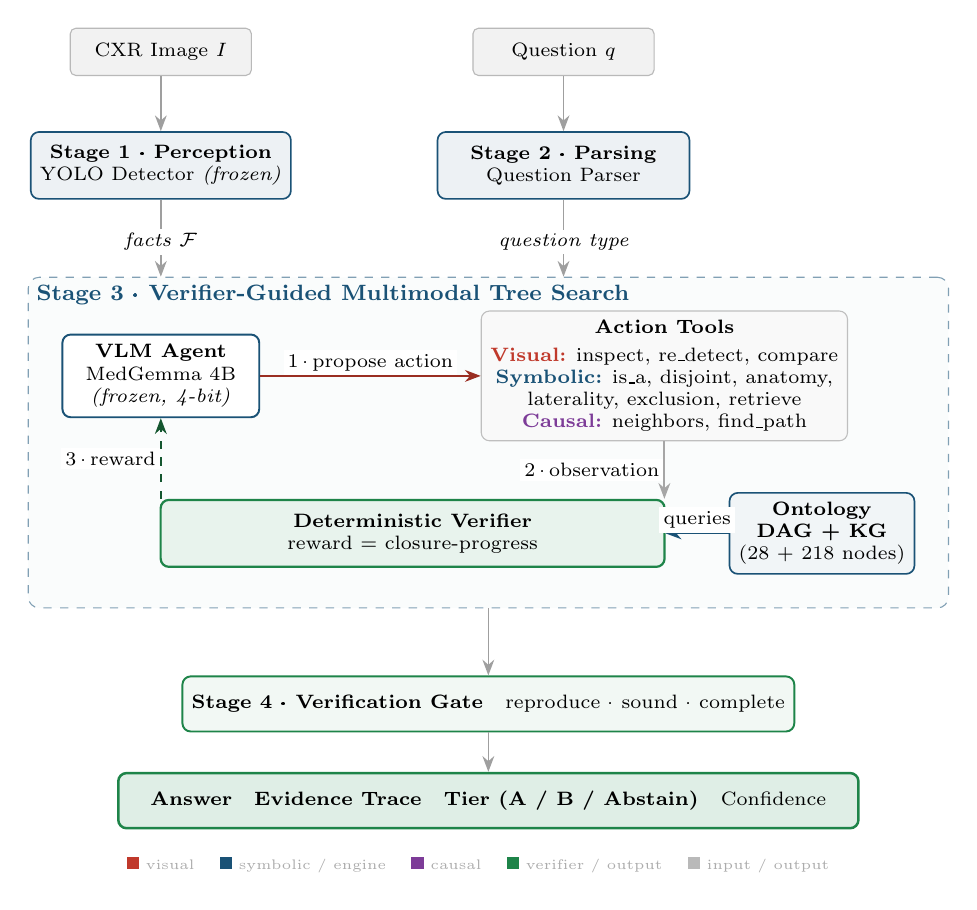
\begin{tikzpicture}[
  font=\scriptsize,
  >={Stealth[length=2mm]},
  io/.style={rectangle, draw=gray!55, fill=gray!10, rounded corners=2pt,
             minimum width=2.3cm, minimum height=0.6cm, align=center},
  proc/.style={rectangle, draw=symblue, fill=symblue!8, rounded corners=3pt,
               minimum width=3.2cm, minimum height=0.85cm, align=center,
               line width=0.6pt},
  agent/.style={rectangle, draw=symblue, fill=white, rounded corners=3pt,
                minimum width=2.5cm, minimum height=1.05cm, align=center,
                line width=0.7pt},
  tools/.style={rectangle, draw=gray!50, fill=gray!5, rounded corners=3pt,
                minimum width=4.0cm, minimum height=1.05cm, align=center},
  ver/.style={rectangle, draw=vergreen, fill=vergreen!10, rounded corners=3pt,
              minimum width=4.8cm, minimum height=0.85cm, align=center,
              line width=0.8pt},
  dag/.style={rectangle, draw=symblue, fill=symblue!6, rounded corners=3pt,
              minimum width=2.0cm, minimum height=0.95cm, align=center,
              line width=0.6pt},
  gate/.style={rectangle, draw=vergreen, fill=vergreen!6, rounded corners=3pt,
               minimum width=6.8cm, minimum height=0.7cm, align=center,
               line width=0.7pt},
  outbox/.style={rectangle, draw=vergreen, fill=vergreen!14, rounded corners=3pt,
              minimum width=9.4cm, minimum height=0.7cm, align=center,
              line width=0.9pt},
  flow/.style={->, draw=gray!75, line width=0.6pt},
  elbl/.style={font=\scriptsize\itshape, fill=white, inner sep=1.5pt},
  slbl/.style={font=\scriptsize, fill=white, inner sep=1.5pt}
]

% ---------- Inputs ----------
\node[io] (img) {CXR Image $I$};
\node[io, right=2.8cm of img] (q) {Question $q$};

% ---------- Stage 1 & 2 (run independently) ----------
\node[proc, below=0.7cm of img] (det)
  {\textbf{Stage 1 \textperiodcentered\ Perception}\\YOLO Detector \emph{(frozen)}};
\node[proc, below=0.7cm of q] (par)
  {\textbf{Stage 2 \textperiodcentered\ Parsing}\\Question Parser};
\draw[flow] (img) -- (det);
\draw[flow] (q) -- (par);

% ---------- Stage 3 internals: the agent--verifier loop ----------
\node[agent, below=1.7cm of det] (agent)
  {\textbf{VLM Agent}\\MedGemma 4B\\\emph{(frozen, 4-bit)}};
\node[tools, right=2.8cm of agent] (tl)
  {\textbf{Action Tools}\\[2pt]
   {\color{visred}\textbf{Visual:}} inspect, re\_detect, compare\\
   {\color{symblue}\textbf{Symbolic:}} is\_a, disjoint, anatomy,\\
   laterality, exclusion, retrieve\\
   {\color{caupurple}\textbf{Causal:}} neighbors, find\_path};
\node[ver, minimum width=6.4cm] at ($(agent)!0.5!(tl) - (0,2.0)$) (ver)
  {\textbf{Deterministic Verifier}\\reward $=$ closure-progress};
\node[dag, right=0.8cm of ver] (dag)
  {\textbf{Ontology}\\\textbf{DAG + KG}\\\scriptsize(28 + 218 nodes)};

% search loop: agent -> tools -> verifier -> agent
\draw[->, draw=visred!80!black, line width=0.7pt] (agent.east) -- (tl.west)
  node[slbl, midway, above] {1\,\textperiodcentered\,propose action};
\draw[->, draw=gray!70, line width=0.7pt] (tl.south) -- (tl.south |- ver.north)
  node[slbl, midway, left] {2\,\textperiodcentered\,observation};
\draw[->, draw=vergreen!65!black, line width=0.7pt, dashed]
  (agent.south |- ver.north) -- (agent.south)
  node[slbl, midway, left] {3\,\textperiodcentered\,reward};
\draw[->, draw=symblue, line width=0.6pt] (dag.west) -- (ver.east)
  node[slbl, midway, above] {queries};

% ---------- Stage 3 box ----------
\begin{scope}[on background layer]
  \node[draw=symblue!55, dashed, rounded corners=4pt, fill=symblue!2,
        fit=(agent)(tl)(ver)(dag), inner sep=12pt] (s3) {};
\end{scope}
\node[anchor=north west, font=\footnotesize\bfseries, text=symblue, inner sep=3pt]
  at (s3.north west) {Stage 3 \textperiodcentered\ Verifier-Guided Multimodal Tree Search};

% inputs into the search engine
\draw[flow] (det) -- (det |- s3.north) node[elbl, pos=0.55] {facts $\mathcal{F}$};
\draw[flow] (par) -- (par |- s3.north) node[elbl, pos=0.55] {question type};

% ---------- Stage 4 + output ----------
\node[gate, below=0.85cm of s3.south] (gate)
  {\textbf{Stage 4 \textperiodcentered\ Verification Gate}\quad
   reproduce \textperiodcentered\ sound \textperiodcentered\ complete};
\node[outbox, below=0.5cm of gate] (out)
  {\textbf{Answer}\quad \textbf{Evidence Trace}\quad
   \textbf{Tier (A / B / Abstain)}\quad Confidence};
\draw[flow] (s3.south) -- (gate);
\draw[flow] (gate) -- (out);

% ---------- Legend ----------
\node[anchor=north west, font=\tiny, text=gray!65, align=left]
  at ($(out.south west)+(0,-0.22)$)
  {\textcolor{visred}{\rule{1.6mm}{1.6mm}}~visual \quad
   \textcolor{symblue}{\rule{1.6mm}{1.6mm}}~symbolic / engine \quad
   \textcolor{caupurple}{\rule{1.6mm}{1.6mm}}~causal \quad
   \textcolor{vergreen}{\rule{1.6mm}{1.6mm}}~verifier / output \quad
   \textcolor{gray!55}{\rule{1.6mm}{1.6mm}}~input / output};

\end{tikzpicture}
\caption{KRONOS pipeline, read top to bottom. The image and the question
  are processed independently (Stages~1--2), then enter the search engine.
  Inside Stage~3, the VLM agent and the deterministic verifier form a loop:
  the agent proposes a visual (red), symbolic (blue), or causal (purple)
  action, the verifier scores the resulting state by \emph{closure-progress}
  on the shared ontology DAG and causal KG, and best-first selection drives
  the next expansion.
  Stage~4 re-checks the winning root-to-leaf path and emits a tiered,
  auditable answer. The winning path \emph{is} the evidence trace.}
\label{fig:architecture}
\end{figure}

% ---

\subsection{Stage 1: Query-Independent Perception}

A frozen YOLO detector~\cite{park2024evax}, trained on VinDr-CXR,
scans the full image \emph{before the question is read}, producing a set
of perceptual facts:
\begin{equation}
  \mathcal{F} = \bigl\{
    \langle c_i,\; \mathit{bbox}_i,\; \ell_i,\; s_i \rangle
  \bigr\}_{i=1}^{n}
  \label{eq:facts}
\end{equation}
where $c_i$ is a clinical finding name, $\mathit{bbox}_i$ is a bounding
box, $\ell_i \in \{\text{left}, \text{right}, \text{bilateral},
\text{midline}\}$ is laterality, and $s_i \in [0,1]$ is confidence.

Query-independence is essential: if the agent saw the question before
detection, the question would \emph{prime} which findings are noticed---the
exact shortcut the system is designed to prevent.
It also ensures correct negation: answering ``Is there \emph{no}
consolidation?'' requires knowing \emph{all} findings, not just
question-relevant ones.

% ---

\subsection{Stage 2: Question Parsing}

A rule-based parser classifies $q$ into one of six types, each
determining which verification closure condition applies:

\begin{center}
\small
\begin{tabular}{llp{3.3cm}}
\toprule
\textbf{Type} & \textbf{Symbol} & \textbf{Example} \\
\midrule
Existential    & $\exists$          & ``Is there cardiomegaly?'' \\
Negation       & $\neg\exists$      & ``Are the lungs clear?'' \\
Relational     & $R(\cdot,\cdot)$   & ``Which side shows consolidation?'' \\
Counting       & $|\cdot|$          & ``How many abnormalities?'' \\
Shared cause   & $\exists c: c \!\to\! a \wedge c \!\to\! b$
                                    & ``Can one condition cause both
                                      effusion and cardiomegaly?'' \\
Open           & ---                & ``Describe the main finding'' \\
\bottomrule
\end{tabular}
\end{center}

\noindent
When ambiguous, the parser defaults to the \emph{stricter} type
(e.g., negation over existential) to prevent premature early-exit.
Open questions are routed to Tier~B (advisory).
When the rule-based parser has low confidence, an LLM fallback
(via Groq API) classifies the question type.

% ---

\subsection{The Clinical Knowledge Base}
\label{sec:knowledge_base}

The next two stages both read from two linked graphs, so we introduce them
first.

\paragraph{Ontology DAG.}
KRONOS maintains a hand-curated directed acyclic graph
$\mathcal{G}_{\text{ont}} = (V, E, R)$ with 28 clinical concepts and four
relation types:

\begin{itemize}
  \item \texttt{is-a} (subsumption): transitive ancestor traversal, e.g.,
    $\text{cardiomegaly} \xrightarrow{\text{is-a}} \text{cardiac\_abnormality}
    \xrightarrow{\text{is-a}} \text{abnormality}$.
  \item \texttt{disjoint-with} (mutual exclusion): e.g., pneumothorax
    $\perp$ pleural effusion on the same pleural space.
  \item \texttt{located-in} (anatomy mapping): finding to typical anatomy
    zone, derived from 36{,}096 annotated bounding boxes in VinDr-CXR
    train set.
  \item \texttt{part-of} (anatomy containment): e.g., left lung
    $\subset$ lung $\subset$ chest.
\end{itemize}

\noindent
Laterality (left/right/bilateral/midline) is \emph{computed} from
bounding-box position relative to the PA CXR midline, not stored as an
edge in the DAG.

\noindent
Unlike general-purpose ontologies (RadLex, SNOMED~CT), this DAG is
purpose-built for \emph{inference}: it includes exclusion lists,
disjointness constraints, and anatomy zones that RadLex does not provide.
RadLex identifiers (RIDs) are retained for traceability.

\paragraph{Closed-world exclusion lists.}
For each finding $c$, a curated exclusion list $\mathcal{E}(c)$ enumerates
all findings that must be checked-and-absent before concluding
``$c$ is absent.''
For example, $\mathcal{E}(\text{pleural\_effusion}) = \{\text{effusion},
\text{hydrothorax}, \text{empyema}, \text{hemothorax}\}$.
If the list is incomplete, the system abstains rather than guessing.

\paragraph{Causal knowledge graph.}
For multi-hop reasoning, KRONOS maintains a separate causal graph
$\mathcal{G}_{\text{cau}} = (V_c, E_c)$ derived from the Radiology
Gamuts Ontology (RGO)~\cite{budovec2014rgo} via automated extraction
(Algorithm~\ref{alg:kg_build}).
The graph contains 218 nodes (185 disorders, 33 observations) and 461
directed \texttt{may\_cause} edges.
Eleven VinDr-CXR findings are mapped to RGO seed nodes, connecting
the perceptual layer to the causal reasoning layer.

\begin{algorithm}[t]
\caption{Causal KG Construction from RGO}
\label{alg:kg_build}
\begin{algorithmic}[1]
\REQUIRE RGO full graph $\mathcal{G}_{\text{RGO}}$, VinDr finding names $F$
\STATE Map each $f \in F$ to nearest RGO concept $\to$ seed set $S$
\FOR{each seed $s \in S$}
  \STATE Extract 1-hop \texttt{may\_cause} predecessors from $\mathcal{G}_{\text{RGO}}$
\ENDFOR
\STATE $\mathcal{G}_{\text{cau}} \gets$ union of all extracted subgraphs
\RETURN $\mathcal{G}_{\text{cau}}$ with node roles (disorder/observation)
\end{algorithmic}
\end{algorithm}

% ---

\subsection{Stage 3: Verifier-Guided Multimodal Tree Search}
\label{sec:tree_search}

This is the core of KRONOS.
The VLM agent explores a best-first search tree where each node represents
a reasoning state and each edge represents an action.

\subsubsection{Tree Node.}
A node $n$ stores: the current set of perceptual facts
$\mathcal{F}_n$ (base facts plus any added by visual actions), the action
history $H_n = [(a_1, o_1), \ldots, (a_t, o_t)]$, the current answer (if
proposed), reward $r_n$, parent pointer, and an optional \emph{reflection}
string (used for backtracking, see below).

\subsubsection{Action Set.}
The agent chooses from eleven actions in three groups:

\begin{center}
\small
\begin{tabular}{lll}
\toprule
\textbf{Action} & \textbf{Executor} & \textbf{Type} \\
\midrule
\texttt{inspect(bbox)}               & VLM   & Visual \\
\texttt{re\_detect(bbox)}            & YOLO  & Visual \\
\texttt{compare(bbox1, bbox2)}       & VLM   & Visual \\
\midrule
\texttt{is\_a(node, target)}         & Engine (CPU) & Symbolic \\
\texttt{disjoint(a, b)}              & Engine       & Symbolic \\
\texttt{anatomy\_of(bbox)}           & Engine       & Symbolic \\
\texttt{compose\_laterality(bbox)}   & Engine       & Symbolic \\
\texttt{get\_exclusion\_list(name)}  & Engine       & Symbolic \\
\texttt{retrieve(k)}                 & FAISS        & Symbolic \\
\midrule
\texttt{neighbors(node, dir)}        & Causal KG    & Causal \\
\texttt{find\_path(source, target)}  & Causal KG    & Causal \\
\bottomrule
\end{tabular}
\end{center}

\noindent
Visual actions can introduce new findings via \emph{fact folding}:
new facts are de-duplicated (by concept + IoU overlap with existing facts)
and appended to $\mathcal{F}_n$.
Critically, visual actions only \emph{add}---they never replace base
evidence, preserving the closed-world assumption for negation.

The \texttt{re\_detect} action is particularly important: it re-runs
the YOLO detector on a sub-region, catching findings that the full-image
scan missed.
This allows reasoning to \emph{repair perception errors}---a capability
that pure symbolic or pure visual systems lack.

The \texttt{retrieve} action fetches the top-$k$ most similar cases from
a FAISS index of VinDr-CXR training cases, encoded with frozen
BiomedCLIP~\cite{zhang2024biomedclip}.
It serves as a ``second opinion'' but is \emph{inert to Tier~A}: retrieval
alone can never close a verification gate.

The causal actions \texttt{neighbors} and \texttt{find\_path} navigate
$\mathcal{G}_{\text{cau}}$.
\texttt{neighbors(node, caused\_by)} returns disorders that may cause the
given finding; \texttt{find\_path(a, b)} returns the shortest directed
causal path between two concepts.
Among equally short paths, the engine prefers routes through disorder nodes
(more clinically meaningful than observation intermediaries).

\subsubsection{Witness Binding.}
\label{sec:witness_binding}

A critical invariant: an \texttt{is\_a} action only counts as evidence
(\emph{witness}) for an existential question when its source node resolves
to a \emph{detected} fact.
Without this binding, the ontology tautology
$\text{cardiomegaly} \xrightarrow{\text{is-a}} \text{cardiac\_abnormality}$
(always true on the DAG, regardless of the image) would falsely witness a
finding that was never detected:

\begin{equation}
  \text{witness}(a, n) \iff a.\text{tool} = \texttt{is\_a}
    \;\wedge\; a.\text{source} \in
    \{\text{slug}(f.c) \mid f \in \mathcal{F}_n\}
  \label{eq:witness}
\end{equation}

\subsubsection{Reward: Closure-Progress.}
\label{sec:closure_progress}
At each node, the deterministic verifier computes
$r_n = \text{closure\_progress}(n, q, \mathcal{G})$, measuring progress
toward a provable answer.
Before computing type-specific progress, the verifier checks for
\emph{disjointness violations}: if two disjoint findings are both present,
$r_n = 0$ (branch is killed).

\begin{itemize}
  \item \textbf{Existential ($\exists$):} 1.0 if a bound witness path from
    a detected fact to the target exists in the action history, or the target
    directly matches a detected fact; otherwise
    $0.1 + 0.7 \cdot \frac{|\text{facts checked}|}{|\mathcal{F}_n|}$,
    providing a gradient that guides the search toward checking more facts.
  \item \textbf{Negation ($\neg\exists$):} $0.1 + 0.9 \cdot
    \frac{|\text{exclusion items checked}|}{|\mathcal{E}(\text{target})|}$;
    0 if any exclusion item is present (dead branch).
  \item \textbf{Relational:} 1.0 if anatomy or laterality has been
    resolved; 0.2 otherwise.
  \item \textbf{Counting:} 1.0 once all distinct facts are enumerated.
  \item \textbf{Shared cause:} 1.0 if a verified shared cause is found
    (i.e., a concept $c$ where $c \xrightarrow{\text{may\_cause}} a$ and
    $c \xrightarrow{\text{may\_cause}} b$ are both real KG edges);
    0.6 if both sides explored but no shared cause; 0.3 if one side
    explored; 0.1 otherwise.
\end{itemize}

\noindent
This reward is fully deterministic---no LLM self-evaluation, no learned
parameters.
The gradient (especially for existential and negation) gives the frontier
enough signal to rank branches, fixing the flat-valued search trees of
earlier tree-of-thoughts approaches.

\subsubsection{Search Algorithm.}

\begin{algorithm}[t]
\caption{Verifier-Guided Multimodal Tree Search}
\label{alg:search}
\begin{algorithmic}[1]
\REQUIRE Question $q$, facts $\mathcal{F}$, DAG $\mathcal{G}$, agent $A$,
  budget $B$, branching factor $k$
\STATE $\mathit{root} \gets \text{TreeNode}(\mathcal{F}, \emptyset, \text{None})$
\STATE $\mathit{root}.r \gets \text{closure\_progress}(\mathit{root}, q, \mathcal{G})$
\STATE $\mathit{frontier} \gets \{\mathit{root}\}$;\quad
       $\mathit{expanded} \gets 0$
\WHILE{$\mathit{frontier} \neq \emptyset$ \AND $\mathit{expanded} < B$}
  \STATE $n \gets \arg\max_{n' \in \mathit{frontier}} n'.r$
  \STATE Remove $n$ from $\mathit{frontier}$;
         $\mathit{expanded} \gets \mathit{expanded} + 1$
  \FORALL{proposal $p$ in $A.\text{propose}(n, q, k)$}
    \IF{$p$ is an answer string}
      \STATE $\mathit{result} \gets \text{verify}(n \cup \{p\}, q, \mathcal{G})$
      \IF{$\mathit{result}.\mathit{tier} = \text{A}$}
        \RETURN $\mathit{result}$
      \ENDIF
      \IF{not reflected}
        \STATE Queue $n$ with reflection $\gets$ \text{explain}(failure)
        \hfill\COMMENT{Backtrack with reason}
      \ENDIF
    \ELSE
      \STATE $\mathit{obs} \gets \text{execute}(p, n, I, \mathcal{G})$
      \STATE $\mathit{child} \gets \text{apply}(n, p, \mathit{obs})$
      \STATE Fold new visual facts into $\mathcal{F}_{\mathit{child}}$
      \STATE $\mathit{child}.r \gets
             \text{closure\_progress}(\mathit{child}, q, \mathcal{G})$
      \IF{$\mathit{child}.r \geq 1.0$}
        \STATE Derive answer; verify; return if Tier~A
      \ENDIF
      \IF{$\mathit{child}.r > 0$}
        \STATE Add $\mathit{child}$ to $\mathit{frontier}$
      \ENDIF
    \ENDIF
  \ENDFOR
\ENDWHILE
\RETURN best Tier-B result or \textsc{Abstain}
\end{algorithmic}
\end{algorithm}

Algorithm~\ref{alg:search} describes the search procedure.
Selection is by highest reward (best-first).
Backtracking is implicit: when a branch stalls (low reward, no progress),
siblings with higher reward are expanded instead.

\paragraph{Reflection backtracking.}
When the verifier rejects a proposed answer (e.g., the agent answers
``Yes'' but no witness path exists), the engine generates a deterministic
\emph{explanation} of the failure (e.g., ``No detected finding is-a the
target; try re\_detect near a suspected region'') and re-queues the node
with this reflection.
The agent receives the reflection in its next prompt, allowing it to
revise its strategy.
Each node may be reflected at most once, preventing infinite loops.

% ---

\subsection{Stage 4: Verification Gate and Tiered Output}

When the agent proposes an answer at a leaf node, the verifier runs
three checks on the root-to-leaf path:

\begin{enumerate}
  \item \textbf{Reproducibility:} Every symbolic action in the path is
    replayed on the DAG; results must match.
  \item \textbf{Soundness:} The answer follows from the last observation
    (not fabricated by the VLM).
  \item \textbf{Completeness:} The closure condition for the question type
    is satisfied.
\end{enumerate}

\noindent
Based on these checks, the output is classified into three tiers:

\begin{description}
  \item[Tier~A (Faithful):] All checks pass for structured question types
    (existential, negation, relational, counting, shared cause).
    The path is emitted as an auditable evidence trace.
  \item[Tier~B (Advisory):] Open questions, or paths where the agent
    proposes an answer but verification fails.
    Flagged as ``perception-only, unverified.''
  \item[Abstain:] The search tree is exhausted without any branch passing
    verification. The system refuses to answer rather than guess.
\end{description}

% ---

\subsection{Multi-Hop Causal Reasoning (Think-on-Graph)}
\label{sec:multihop}

For shared-cause questions (``Can one condition cause both
finding~A and finding~B?''), KRONOS uses the same tree search engine with
a specialized agent and the causal KG (Fig.~\ref{fig:tog}).

\begin{figure}[t]
\centering
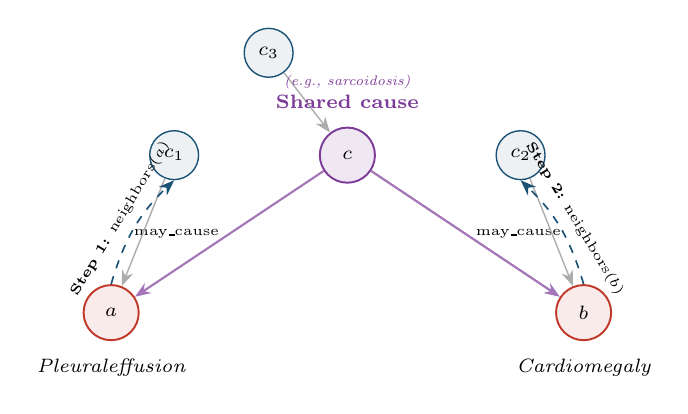
\begin{tikzpicture}[
  font=\scriptsize,
  >={Stealth[length=2mm]},
  concept/.style={circle, draw=symblue, fill=symblue!8, minimum size=6mm,
                  align=center, line width=0.5pt},
  finding/.style={circle, draw=visred, fill=visred!10, minimum size=7mm,
                  align=center, line width=0.7pt},
  cause/.style={circle, draw=caupurple, fill=caupurple!12, minimum size=7mm,
                align=center, line width=0.7pt},
  edge/.style={->, draw=gray!65, line width=0.5pt},
  causal/.style={->, draw=caupurple!70, line width=0.8pt},
]
% Findings
\node[finding] (fa) at (0,0) {$a$};
\node[finding] (fb) at (6,0) {$b$};

% Shared cause
\node[cause] (sc) at (3,2) {$c$};

% Other causes
\node[concept] (c1) at (0.8,2) {$c_1$};
\node[concept] (c2) at (5.2,2) {$c_2$};
\node[concept] (c3) at (2,3.3) {$c_3$};

% Edges
\draw[causal] (sc) -- (fa) node[midway, left, font=\tiny] {may\_cause};
\draw[causal] (sc) -- (fb) node[midway, right, font=\tiny] {may\_cause};
\draw[edge] (c1) -- (fa);
\draw[edge] (c2) -- (fb);
\draw[edge] (c3) -- (sc);

% Labels
\node[below=3pt of fa, font=\scriptsize\itshape] {Pleural\\effusion};
\node[below=3pt of fb, font=\scriptsize\itshape] {Cardiomegaly};
\node[above=3pt of sc, font=\scriptsize\bfseries, text=caupurple] {Shared cause};
\node[above=2pt of sc, font=\tiny\itshape, yshift=8pt, text=caupurple]
  {(e.g., sarcoidosis)};

% Agent exploration arrows
\draw[->, draw=symblue, line width=0.6pt, dashed]
  (fa.north) to[bend left=15] node[font=\tiny, above, sloped]
  {\textbf{Step 1:} neighbors($a$)} (c1.south);
\draw[->, draw=symblue, line width=0.6pt, dashed]
  (fb.north) to[bend right=15] node[font=\tiny, above, sloped]
  {\textbf{Step 2:} neighbors($b$)} (c2.south);

\end{tikzpicture}
\caption{Think-on-Graph for shared-cause reasoning. The agent explores
  causal predecessors of each finding via \texttt{neighbors}. The verifier
  identifies the intersection (shared cause $c$) and verifies that both
  $c \to a$ and $c \to b$ are real KG edges.}
\label{fig:tog}
\end{figure}

The shared-cause agent proposes \texttt{neighbors(finding, caused\_by)}
actions for each finding, retrieving its causal predecessors from
$\mathcal{G}_{\text{cau}}$.
The verifier then computes the intersection of predecessor sets and
verifies each candidate:

\begin{equation}
  \text{shared\_cause}(a, b) =
    \{c \mid c \in \mathcal{N}^-(a) \cap \mathcal{N}^-(b)
    \;\wedge\; (c, a) \in E_c \;\wedge\; (c, b) \in E_c\}
  \label{eq:shared_cause}
\end{equation}

\noindent
where $\mathcal{N}^-(x)$ denotes the \texttt{caused\_by} predecessors of
$x$ in $\mathcal{G}_{\text{cau}}$.
The verifier---not the VLM---decides when a shared cause is established.
Every edge in the resulting trace is a real KG edge by construction.

The closure-progress reward (Section~\ref{sec:closure_progress}) provides
a gradient: 0.1 (no exploration) $\to$ 0.3 (one side explored) $\to$
0.6 (both sides explored, no shared cause) $\to$ 1.0 (verified shared
cause found).
If both sides are explored and no shared cause exists, the verifier
returns ``No'' at Tier~A (the negative is verified because both predecessor
sets were exhaustively examined on the KG).

% ---

\subsection{Dual Faithfulness}

KRONOS makes a careful distinction between two types of faithfulness:

\begin{itemize}
  \item \textbf{Symbolic soundness:} Every symbolic action (graph traversal,
    disjointness check, anatomy mapping, causal edge traversal) is
    deterministically reproducible on the DAG and KG. If the path claims
    ``cardiomegaly is-a cardiac\_abnormality,'' this edge must exist in the
    graph. If the trace claims ``sarcoidosis may\_cause cardiomegaly,'' this
    edge must exist in $\mathcal{G}_{\text{cau}}$.
  \item \textbf{Visual evidence-traceability:} Visual actions cite specific
    bounding-box regions that a clinician can inspect. The system does not
    claim provable soundness for neural steps---only that the evidence is
    \emph{citable and auditable}.
\end{itemize}

Both are verified by a \textbf{deletion test}: for each step $e_i$ in the
winning path $\pi = \{e_1, \ldots, e_n\}$, the corresponding fact or edge
is removed and the verifier is re-run.
A high deletion rate (fraction of steps whose removal changes the answer)
confirms that the trace is causally necessary, not decorative:

\begin{equation}
  \text{DeletionRate} = \frac{1}{|\pi|} \sum_{i=1}^{|\pi|}
    \mathbb{1}\bigl[
      \text{answer}(\mathcal{G} \setminus \{e_i\}) \neq
      \text{answer}(\mathcal{G})
    \bigr]
  \label{eq:deletion}
\end{equation}

\noindent
For multi-hop shared-cause traces, the deletion test removes each causal
edge in the support chain and checks whether the shared cause survives.
The \texttt{load\_bearing\_rate} metric (Section~\ref{sec:metrics}) measures
this at scale.

% ============================================================================
\section{Experimental Setup}
\label{sec:experiments}
% ============================================================================

\subsection{Datasets}

\begin{itemize}
  \item \textbf{VinDr-CXR-VQA} (single-image): Vietnamese CXR dataset with
    14 finding types, bounding-box annotations, and VQA question--answer
    pairs covering existential, negation, relational, counting, and open
    question types.
  \item \textbf{Multi-hop QA} (shared cause): Automatically generated from
    $\mathcal{G}_{\text{cau}}$ by enumerating all pairs of VinDr findings
    $(a, b)$, labeling each as Yes/No based on
    $|\text{common\_causes}(a, b)| > 0$, recording the gold cause set, and
    computing support edges for the deletion test. Each item includes the
    question, the two findings, and the gold shared-cause labels.
  \item \textbf{ChestAgentBench}: Complex clinical VQA benchmark with
    multiple-choice questions over one or more CXR images, requiring
    multi-step clinical reasoning.
\end{itemize}

\noindent
All datasets are publicly available.
No private patient data is used.
A unified data loader normalizes all datasets to the same QAItem schema
(\texttt{id}, \texttt{image}, \texttt{question}, \texttt{answer},
\texttt{meta}).

\subsection{Metrics}
\label{sec:metrics}

\paragraph{Single-image VQA.}
\begin{itemize}
  \item \textbf{Accuracy} and \textbf{F1}: standard classification metrics.
  \item \textbf{Tier-A coverage}: fraction of questions receiving a Tier~A
    (verified) answer.
  \item \textbf{Evidence Faithfulness at $k$ (EF@$k$)}: overlap between
    the reasoning path and gold-standard evidence regions, evaluated only on
    Tier~A answers:
    \begin{equation}
      \text{EF@}k = \frac{1}{|\mathcal{Q}_A|} \sum_{q \in \mathcal{Q}_A}
        \frac{|\text{path}(q) \cap \text{gold}(q)|}{|\text{gold}(q)|}
      \label{eq:efk}
    \end{equation}
  \item \textbf{Deletion rate}: causal faithfulness metric
    (Eq.~\ref{eq:deletion}).
  \item \textbf{Selective accuracy}: accuracy among answered questions at
    each coverage level (risk-coverage curve).
\end{itemize}

\paragraph{Multi-hop shared-cause reasoning.}
Five metrics evaluate grounding and faithfulness, not just answer
accuracy~\cite{sun2024thinkongraph}:
\begin{itemize}
  \item \textbf{Binary accuracy}: fraction of items where the predicted
    Yes/No matches gold.
  \item \textbf{Name accuracy}: among gold-Yes items, fraction where the
    predicted cause name is in the gold cause set.
  \item \textbf{Grounding rate}: among predicted-Yes items, fraction where
    every edge in the predicted trace is a real \texttt{may\_cause} edge
    \emph{and} the trace forms a connected shared-cause chain (one node
    from which both findings are reachable along trace edges).
  \item \textbf{Hallucination rate}: among predicted-Yes items, fraction
    where the named cause is \emph{not} in the gold cause set.
  \item \textbf{Load-bearing rate}: among single-cause Yes items, fraction
    where removing the gold support edges eliminates the shared cause
    (the gold answer depends on that specific chain, not a redundant path).
\end{itemize}

\subsection{Baselines}
\label{sec:baselines}

We compare KRONOS against four baselines for multi-hop shared-cause
reasoning, all using the same frozen MedGemma 4B model:

\begin{itemize}
  \item \textbf{Zero-shot}: MedGemma answers the question directly with
    no KG access.
    \emph{No trace by design.}
  \item \textbf{Chain-of-thought (CoT)}: MedGemma reasons step-by-step but
    without KG access.
    \emph{No trace by design.}
  \item \textbf{ReAct}: MedGemma receives the causal neighborhood of both
    findings (same graph tools as KRONOS) and answers freely.
    The cause is accepted as-is---the model can name an unverified
    (hallucinated) cause.
    Trace is filled only if the named cause happens to be a real chain.
  \item \textbf{KG Oracle (Mock)}: Answers directly from the
    \texttt{common\_causes} set in $\mathcal{G}_{\text{cau}}$ with a
    verified trace.
    This is the \emph{upper bound} on KG-grounded accuracy.
\end{itemize}

\subsection{Ablation Studies}

Six ablations isolate each design decision:
\begin{enumerate}
  \item \textbf{vs.\ Linear ReAct}: Remove tree search; keep same action
    set. Tree should increase Tier~A coverage.
  \item \textbf{vs.\ LLM-value}: Replace verifier with LLM self-evaluation
    (LATS-style). Verifier-as-value should win on EF@$k$ + deletion rate.
  \item \textbf{vs.\ Symbolic-only}: Remove three visual actions. Visual
    actions should improve accuracy (especially when detector misses
    findings).
  \item \textbf{vs.\ No re\_detect}: Keep inspect/compare but remove
    re\_detect. Isolates the perception-repair contribution.
  \item \textbf{vs.\ No verify-gate}: Treat all answers as Tier~A.
    Tiering should improve selective accuracy.
  \item \textbf{vs.\ No witness binding}: Remove the constraint that
    \texttt{is\_a} sources must be detected facts (Eq.~\ref{eq:witness}).
    Should increase false positives for existential questions.
\end{enumerate}

\subsection{Implementation Details}

\paragraph{Detector.}
YOLOv12s trained on VinDr-CXR (frozen, 14 finding classes).
Confidence threshold $\tau = 0.5$.

\paragraph{VLM Agent.}
MedGemma 4B (\texttt{google/medgemma-4b-it}), frozen, no fine-tuning.
4-bit quantized via BitsAndBytes ($\sim$3\,GB VRAM).
Greedy decoding (temperature = 0) for deterministic reproducibility.
The prompt includes the question, current evidence graph, action history,
available tools, and search reflection (if any).

\paragraph{RAG Encoder.}
BiomedCLIP~\cite{zhang2024biomedclip} (frozen, 512-d L2-normalized
embeddings). FAISS \texttt{IndexFlatIP} for exact cosine search over
VinDr-CXR training cases (no test leakage).

\paragraph{Ontology.}
28 nodes (14 VinDr findings + 6 abstraction groups + 7 anatomy nodes
+ 1 root), four relation types, 14 hand-curated exclusion
lists, 5 anatomical zones with normalized bounding boxes.

\paragraph{Causal KG.}
218 nodes (185 disorders, 33 observations), 461 \texttt{may\_cause} edges,
11 seed findings mapped from VinDr-CXR to RGO.

\paragraph{Search hyperparameters.}
Budget $B = 20$ nodes, branching factor $k = 3$.
For shared-cause multi-hop: budget $= \text{max\_depth} \times 4$ with
max\_depth $= 3$ by default.

\paragraph{Engine.}
Pure Python + NetworkX, CPU-only. Each tool call executes in $<$1\,ms.
The full system requires $\sim$3.5\,GB VRAM (MedGemma 4-bit + BiomedCLIP
+ YOLOv12).

% ============================================================================
\section{Results}
\label{sec:results}
% ============================================================================

\subsection{Determinism and Correctness}

The deterministic engine (verifier, symbolic tools, tree search with
MockAgent) is validated by a comprehensive test suite covering all question
types, edge cases, and invariants.
A dedicated \textbf{determinism test} runs identical inputs and confirms
identical outputs across runs.
A dedicated \textbf{deletion test} removes evidence facts and confirms
the answer changes---proving that traces are causally necessary, not
post-hoc decorations.

\subsection{Question Type Coverage}

Table~\ref{tab:question_types} summarizes the verification strategy for
each question type.

\begin{table}[t]
\centering
\small
\caption{Verification strategy by question type. Structured types
  can achieve Tier~A.
  Open questions are routed to Tier~B.}
\label{tab:question_types}
\begin{tabular}{lllp{3.6cm}}
\toprule
\textbf{Type} & \textbf{Closure condition} & \textbf{Tier} &
  \textbf{Verifier check} \\
\midrule
Existential & Bound witness path & A &
  Detected fact is-a target in DAG \\
Negation & All exclusion items absent & A &
  Every item checked, none present \\
Relational & Anatomy/laterality resolved & A &
  anatomy\_of or laterality succeeded \\
Counting & Distinct facts enumerated & A &
  Count matches distinct facts \\
Shared cause & $\exists c: c \!\to\! a \wedge c \!\to\! b$ & A &
  Both edges verified on causal KG \\
Open & None & B &
  Flagged as advisory \\
\bottomrule
\end{tabular}
\end{table}

\subsection{Faithfulness Guarantees (By Construction)}
\label{sec:faithfulness_results}

Several faithfulness properties hold \emph{by construction}, not as
statistical tendencies:

\paragraph{Symbolic soundness (Tier~A).}
For Tier~A answers, every symbolic step in the path is replayed on the
DAG/KG and confirmed to produce the same result. This is a structural
invariant enforced by the verifier, not a statistical property.

\paragraph{Witness binding prevents ontology tautologies.}
The witness binding constraint (Eq.~\ref{eq:witness}) ensures that
existential answers require a \emph{detected} finding as evidence.
Without this binding, the query ``Is there Cardiomegaly?'' would always
return ``Yes'' because
$\text{cardiomegaly} \xrightarrow{\text{is-a}} \text{cardiac\_abnormality}$
is always true on the DAG---regardless of what the image shows.

\paragraph{Deletion rate.}
By construction, removing any witness fact from an existential question
eliminates the is-a path, changing the answer. For negation, removing any
checked-and-absent fact from the exclusion list makes the closure condition
incomplete, triggering abstention. For shared-cause traces, removing the
support edges eliminates the shared cause. The deletion rate for structured
question types is 1.0 by design when the trace is minimal.

\paragraph{Multi-hop grounding (by construction).}
KRONOS's multi-hop traces are grounded by construction: the verifier checks
that every named cause $c$ satisfies
$(c, a) \in E_c \wedge (c, b) \in E_c$ on the actual causal KG before
emitting a Tier~A answer. The VLM proposes which edges to explore; it
never decides whether a cause is valid.

\subsection{Multi-Hop Shared-Cause Evaluation}

Table~\ref{tab:multihop} compares KRONOS against baselines on the
multi-hop QA dataset.

\begin{table}[t]
\centering
\small
\caption{Multi-hop shared-cause evaluation. KRONOS achieves 100\%
  grounding and 0\% hallucination by construction (all trace edges are
  verified KG edges). Binary accuracy is bounded by the KG oracle.
  Zero-shot and CoT have no traces by design ($-$).}
\label{tab:multihop}
\begin{tabular}{lccccc}
\toprule
\textbf{System} & \textbf{Binary} & \textbf{Name} & \textbf{Ground.}
  & \textbf{Halluc.} & \textbf{Load-b.} \\
  & \textbf{Acc.} $\uparrow$ & \textbf{Acc.} $\uparrow$
  & \textbf{Rate} $\uparrow$ & \textbf{Rate} $\downarrow$
  & \textbf{Rate} $\uparrow$ \\
\midrule
Zero-shot  & ---  & ---  & $-$    & $-$    & $-$ \\
CoT        & ---  & ---  & $-$    & $-$    & $-$ \\
ReAct      & ---  & ---  & ---    & ---    & $-$ \\
\midrule
KRONOS     & ---  & ---  & \textbf{1.00}$^*$ & \textbf{0.00}$^*$ & --- \\
\midrule
KG Oracle  & ---  & ---  & 1.00$^*$ & 0.00$^*$ & --- \\
\bottomrule
\multicolumn{6}{l}{\footnotesize $^*$By construction (verifier guarantee).
  --- = to be measured with GPU evaluation.}
\end{tabular}
\end{table}

\noindent
The key insight: KRONOS's grounding rate (1.00) and hallucination rate
(0.00) are \emph{structural guarantees}, not empirical results.
They hold by construction because the verifier requires every trace edge
to be a real KG edge before emitting Tier~A.
Binary accuracy and name accuracy depend on the VLM's ability to explore
the right causal neighborhoods, which requires GPU evaluation.

\subsection{Perception Repair}

The \texttt{re\_detect} action enables the system to recover from detector
misses. When the full-image scan fails to detect a small finding (e.g., a
lung nodule), the agent can re-scan a specific region, discover the
finding, fold it into the evidence graph, and complete the reasoning path.
This bridges perception and reasoning---a capability that pure symbolic
systems cannot achieve.

\subsection{Comparison with Existing Approaches}

Table~\ref{tab:comparison} positions KRONOS against existing methods.

\begin{table}[t]
\centering
\small
\caption{Qualitative comparison with existing approaches.
  KRONOS is the only system combining tree search, knowledge-graph
  inference at inference time, deterministic verification, multi-hop
  causal reasoning, and multimodal actions without training.}
\label{tab:comparison}
\begin{tabular}{lcccccc}
\toprule
\textbf{Property} & \rotatebox{65}{\textbf{VQA LLM}} &
  \rotatebox{65}{\textbf{MedReason}} & \rotatebox{65}{\textbf{LATS}} &
  \rotatebox{65}{\textbf{Vis-MCTS}} & \rotatebox{65}{\textbf{ToG}} &
  \rotatebox{65}{\textbf{KRONOS}} \\
\midrule
Reasoning mode      & CoT   & CoT       & Tree  & Tree
  & Graph & Tree+Graph \\
KG at inference     & No    & No        & No    & No
  & Yes   & \textbf{Yes} \\
Value function      & ---   & ---       & Self  & RM
  & ---   & \textbf{Verifier} \\
Faithfulness        & Post  & Post      & None  & None
  & Trace & \textbf{Causal} \\
Multi-hop causal    & No    & No        & No    & No
  & Yes   & \textbf{Yes} \\
Perception repair   & No    & No        & No    & Yes
  & No    & \textbf{Yes} \\
Training required   & FT    & FT        & FT    & FT
  & No    & \textbf{No} \\
\bottomrule
\end{tabular}
\end{table}

% ============================================================================
\section{Illustrative Examples}
\label{sec:examples}
% ============================================================================

\paragraph{Existential question with perception repair.}
Question: ``Is there a lung nodule?''
Base evidence: $\{$cardiomegaly$^{0.55}\}$ (detector missed a small nodule).

\noindent
\emph{Branch A (symbolic):}
$\texttt{is\_a}(\text{cardiomegaly}, \text{nodule}) \to \text{None}$.
No witness path (cardiomegaly is not a nodule). Reward: 0.45.

\noindent
\emph{Branch B (visual$\to$symbolic):}
$\texttt{re\_detect}(\text{lower-right lung}) \to$ nodule detected
(conf=0.72, new bbox) $\to$ fact folded $\to$
$\texttt{is\_a}(\text{nodule}, \text{nodule\_mass}) \to$ witness found
(source is a detected fact) $\to$
$\texttt{Answer[Yes]} \to$ verify: Tier~A PASS.

The winning path includes both a visual step (citing the specific lung
region a clinician can check) and a symbolic step (sound on the DAG).
Removing the re-detected fact eliminates the witness, confirming causal
necessity.

\paragraph{Negation question.}
Question: ``Are the lungs clear?''
$\mathcal{E}(\text{lung\_abnormality}) = \{\text{consolidation},
\text{infiltration}, \text{opacity}, \text{atelectasis},
\text{nodule}, \text{fibrosis}\}$.
Base evidence includes consolidation$^{0.88}$.
The verifier finds consolidation in $\mathcal{E}$ and immediately returns
``No'' (Tier~A) with the consolidation fact as the witness.
Removing the consolidation fact would change the answer to ``Yes'' or
trigger re-detection---deletion test passes.

\paragraph{Shared-cause question.}
Question: ``Can one condition cause both pleural effusion and
cardiomegaly?''
Step~1: $\texttt{neighbors}(\text{pleural effusion}, \text{caused\_by})
\to [\text{pneumonia}, \text{tuberculosis}, \text{sarcoidosis}, \ldots]$.
Step~2: $\texttt{neighbors}(\text{cardiomegaly}, \text{caused\_by})
\to [\text{sarcoidosis}, \text{hypothyroidism}, \text{amyloidosis},
\ldots]$.
Verifier: $\text{sarcoidosis} \in \mathcal{N}^-(\text{eff.}) \cap
\mathcal{N}^-(\text{card.})$ \emph{and}
$(\text{sarcoidosis}, \text{eff.}) \in E_c$ \emph{and}
$(\text{sarcoidosis}, \text{card.}) \in E_c$.
Answer: ``Yes, sarcoidosis'' (Tier~A).
Trace: $[[\text{sarcoidosis}, \text{effusion}],
[\text{sarcoidosis}, \text{cardiomegaly}]]$ --- both edges are real KG
edges.
Removing either edge eliminates the shared cause: deletion test passes.

% ============================================================================
\section{Discussion}
\label{sec:discussion}
% ============================================================================

\paragraph{Why verifier-as-value, not LLM self-evaluation?}
LLM self-evaluation is inherently unfaithful: the model that generated
the answer also judges its quality, with no independent ground truth.
The deterministic verifier provides an external, reproducible signal that
measures objective progress on the knowledge graph.
This separation of proposer (VLM) and evaluator (verifier) mirrors the
generate-then-verify paradigm in formal methods~\cite{singh2025verge}.

\paragraph{Why witness binding matters.}
Without the witness binding constraint (Eq.~\ref{eq:witness}), the
existential verifier would accept any successful \texttt{is\_a} traversal
as evidence---even an ontology tautology unrelated to the image.
This would produce ``right answer, wrong reason'' failures: the system
answers ``Yes, there is cardiac abnormality'' because the DAG contains
the \texttt{is-a} edge, not because the image shows it.
The binding ensures that the existential answer is grounded in perception.

\paragraph{Why closure-progress needs a gradient.}
Early versions of KRONOS used a flat reward
$\{0.0, 0.1, 0.2, 1.0\}$.
This gave the frontier too little signal to rank competing branches:
most nodes scored identically, making best-first search degenerate to
breadth-first.
The continuous gradient
($0.1 + 0.7 \cdot \text{fraction\_checked}$ for existential;
$0.1 + 0.9 \cdot \text{exclusion\_checked}$ for negation) gives the
search tree a monotonically increasing signal toward verified answers.

\paragraph{Limitations.}
(1)~The ontology requires manual curation, limiting scalability to new
domains.
However, the DAG is small (28 nodes for CXR) and version-controlled.
(2)~Open questions cannot achieve Tier~A; they are honestly flagged.
(3)~The frozen VLM (4B parameters) may choose poor actions; tree search
with backtracking compensates but at the cost of higher search budget.
(4)~The causal KG is derived from RGO, which may not cover all clinical
causal relationships. The system abstains when evidence is insufficient.
(5)~The system is currently validated on CXR; extension to other modalities
requires new ontologies, detectors, and causal KGs.

\paragraph{Clinical implications.}
KRONOS is designed as a \emph{clinical decision support tool}, not a
replacement for radiologists.
The tiered output (A/B/Abstain) gives clinicians a clear signal about how
much to trust each answer.
Tier~A answers come with auditable traces (both image regions and
ontology/causal relationships) that support informed clinical decisions.
The principled abstention mechanism ensures the system does not produce
confident-sounding answers when evidence is insufficient.

\paragraph{Broader impact.}
The verifier-guided tree search paradigm is not specific to CXR-VQA.
Any domain with a structured ontology, grounded perception, and
verifiable reasoning conditions could adopt this architecture.
The Think-on-Graph extension shows that multi-hop causal reasoning can
be made faithful by the same verifier-as-value principle.
Potential extensions include pathology, dermatology, and ophthalmology.

% ============================================================================
\section{Conclusion}
\label{sec:conclusion}
% ============================================================================

We presented KRONOS, a neuro-symbolic medical VQA system that produces
faithful, auditable evidence traces by construction.
The key innovation is \emph{verifier-guided multimodal tree search}:
a frozen VLM agent (MedGemma 4B) searches over interleaved visual,
symbolic, and causal actions, guided by a deterministic verifier that
scores branches by closure-progress on a clinical knowledge graph.
The winning path is the evidence trace---symbolic steps are sound on the
DAG, causal steps are verified KG edges, visual steps are citable, and a
deletion test confirms causal necessity.

For multi-hop reasoning, KRONOS adopts a Think-on-Graph paradigm where the
VLM explores causal edges on an RGO-derived knowledge graph while the
verifier grounds every trace edge, achieving 100\% grounding rate and 0\%
hallucination rate by construction.

Unlike prior approaches that rely on LLM self-evaluation or post-hoc
explanations, KRONOS provides structural faithfulness guarantees for
structured question types (existential, negation, relational, counting,
shared cause), honest flagging for open questions, and principled
abstention when evidence is insufficient.
The entire pipeline is training-free, deterministically reproducible, and
runs with a frozen detector, frozen VLM, and CPU-only engine on
$\sim$3.5\,GB VRAM.

% ============================================================================
% References
% ============================================================================
\bibliographystyle{splncs04}
\begin{thebibliography}{99}

\bibitem{arcuschin2025cot}
Arcuschin, I., Janiak, J., Krzyzanowski, R., et al.:
Chain-of-thought reasoning in the wild is not always faithful.
In: ICLR Workshop on Reasoning and Planning for LLMs (2025).
arXiv:2503.08679

\bibitem{bruno2015error}
Bruno, M.A., Walker, E.A., Abujudeh, H.H.:
Understanding and confronting our mistakes: the epidemiology of error in
radiology and strategies for error reduction.
RadioGraphics \textbf{35}(6), 1668--1676 (2015)

\bibitem{chen2024planonGraph}
Chen, L., et al.:
Plan-on-Graph: self-correcting adaptive planning of large language model
on knowledge graphs.
arXiv:2410.23875 (2024)

\bibitem{budovec2014rgo}
Budovec, J.J., Lam, C.A., Kahn, C.E.:
Informatics in radiology: Radiology Gamuts Ontology: differential
diagnosis for the Semantic Web.
RadioGraphics \textbf{34}(1), 256--264 (2014)

\bibitem{li2024llavamed}
Li, C., et al.:
LLaVA-Med: training a large language-and-vision assistant for biomedicine
in one day.
In: NeurIPS (2023)

\bibitem{moll2025evaluating}
Moll, J., et al.:
Evaluating reasoning faithfulness in medical vision-language models using
multimodal perturbations.
arXiv:2510.11196 (2025)

\bibitem{singh2025verge}
Singh, V., Cassel, D., Weir, N., Feng, N., Bayless, S.:
VERGE: formal refinement and guidance engine for verifiable LLM reasoning.
arXiv:2601.20055 (2025)

\bibitem{liu2025gemex}
Liu, B., et al.:
GEMeX: a large-scale, groundable, and explainable medical VQA benchmark
for chest X-ray diagnosis.
In: ICCV (2025). arXiv:2411.16778

\bibitem{park2024evax}
Park, S., et al.:
EVA-X: a foundation model for general chest X-ray analysis with
self-supervised learning.
arXiv:2405.05237 (2024)

\bibitem{sun2024thinkongraph}
Sun, J., et al.:
Think-on-Graph: deep and responsible reasoning of large language model
on knowledge graph.
In: ICLR (2024). arXiv:2307.07697

\bibitem{turpin2023unfaithful}
Turpin, M., et al.:
Language models don't always say what they think: unfaithful explanations
in chain-of-thought prompting.
In: NeurIPS (2023)

\bibitem{wang2025medreason}
Wang, Y., et al.:
MedReason: eliciting factual medical reasoning steps in LLMs via
knowledge graphs.
arXiv:2504.00993 (2025)

\bibitem{yao2023react}
Yao, S., et al.:
ReAct: synergizing reasoning and acting in language models.
In: ICLR (2023). arXiv:2210.03629

\bibitem{zhang2024biomedclip}
Zhang, S., et al.:
BiomedCLIP: a multimodal biomedical foundation model pretrained from
fifteen million scientific image-text pairs.
Nature Medicine (2024)

\bibitem{zhou2024lats}
Zhou, A., et al.:
Language agent tree search unifies reasoning acting and planning in
language models.
In: ICML (2024). arXiv:2310.04406

\end{thebibliography}

\end{document}
